To be able to write a paper with \LaTeX\ you need three things.

\begin{enumerate}
\item A \LaTeX distribution
  \begin{compactitem}
  \item \TeX\ Live (\url{https://www.tug.org/texlive/}, all platforms, recommended)
  \item MiK\TeX\ (\url{http://miktex.org/}, Windows only)
  \end{compactitem}

\item Any text editor or a special \LaTeX editor.
  \begin{compactitem}
  \item \TeX studio (\url{http://texstudio.sourceforge.net/})
  \item \TeX works (\url{http://www.tug.org/texworks/})
  \item Kile (\url{http://kile.sourceforge.net/})
  \item \TeX nicCenter (\url{http://www.texniccenter.org/})
  \item Texmaker (\url{http://www.xm1math.net/texmaker/})
  \item LEd (\url{http://www.latexeditor.org/})
  \end{compactitem}

\item A PDF document viewer
  \begin{compactitem}
  \item Eyepiece (\url{http://okular.kde.org/})
  \item Evince (\url{https://wiki.gnome.org/Apps/Evince})
  \item Adobe Acrobat (\url{http://get.adobe.com/de/reader/})
  \end{compactitem}
\end{enumerate}


The \LaTeX compiler translates the manuscript written by the author into a
displayable PDF file. In the past, the output was still in DVI format, which
had to be converted to PDF via intermediate stages. But this is no longer the
case.

The translation process is shown in Figure~\ref{fig:intro:compile}.
In addition to the output PDF, a log file is created with the extension \texttt{.log},
which contains notes, warnings or error messages.
Furthermore, various temporary files are created, which are used for the
directories and for cross-references in the document. The files have different
extensions. As an example the \texttt{.aux} files are mentioned here as an example.
The author does not have to worry about these files.


\begin{figure}
\centering
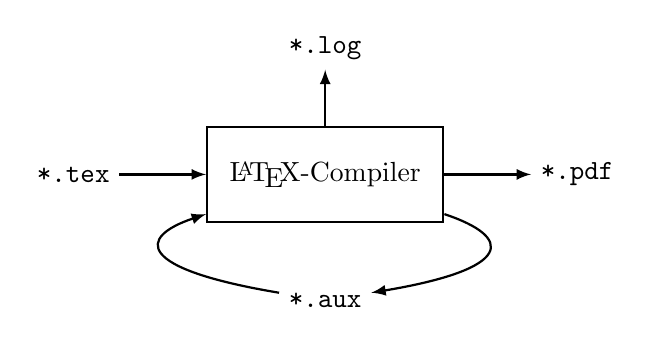
\begin{tikzpicture}[scale=0.8]
\node (latex) at ( 0.0,  0.0) [draw,thick,minimum width=3cm,minimum height=1.2cm] {\LaTeX-Compiler};
\node (tex)   at (-4.0,  0.0) {\texttt{*.tex}};
\node (log)   at ( 0.0,  2.0) {\texttt{*.log}};
\node (aux)   at ( 0.0, -2.0) {\texttt{*.aux}};
\node (pdf)   at ( 4.0,  0.0) {\texttt{*.pdf}};

\draw [-latex,thick] (tex)   -- (latex);
\draw [-latex,thick] (latex) -- (pdf);
\draw [-latex,thick] (latex) -- (log);
\draw [-latex,thick] (latex) .. controls ( 3, -1.0) and ( 3, -1.5) .. (aux);
\draw [-latex,thick] (aux)   .. controls (-3, -1.5) and (-3, -1.0) .. (latex);
\end{tikzpicture}
\caption{Simplified flow of the \LaTeX translation process}
\label{fig:intro:compile}
\end{figure}
